\chapter{Inpainting Sparse Sampled Epipolar-plane and Computing Depth Map}
\label{chap:Inpainting_sparse}

We just presented in Subsection~\ref{sec:shearlet_parseval_inpainting} a general framework for image inpainting using Parseval Frames and we also presented the comparison of general Shearlet Parseval Frames (which include Universal Shearlets, $\alpha$-Shearlets and Cone Adapted Shearlets) and Wavelet Parseval Frames in the task of inpainting a line-distribution singularity, having the conclusion that Shearlets are better by its directional sensitivity.

\bigskip

We also presented in Subsection~\ref{sec:0-Shearlets} the particular case of Universal Shearlets with scaling sequence given by the parameters $\alpha_j=-2/j$, which generates a Parseval frame that is a good choice for the represenation of singularities distributed over straight lines, and therefore is a good option for inpainting Epipolar Plane Images that are formed by linear structures.

\bigskip

In this chapter we will present a particular algorithm that we used to inpaint EPIs related to sparse sampled light fields using $0$-Shearlets in the Julia implemenation of Shearlab (Shearlab.jl) which is called Iterative Hard Thresholding; we will also present the results on the impainting for a particular data set (the Church Data set already mentioned in Chapter 2). 

\bigskip

Using the inpainted EPIs we will present a line detection algorithm called Hough Line Transform that allows us to get the slopes of the lines related to different features in in the EPIs and therefore let us compute the depth map of the scene concluding the light field reconstruction task that we were looking for in this thesis. 

\section{Iterative thresholding algorithm for EPIs inpainting using $0$-Shearlets}

To formulate the light field reconstruction algorithm in discrete domain we will assume that that the starting coarse set of views is a downsampled version of the unknown densely sampled light field we are trying to reconstruct. The uniformly distributed cameras imply the possibility of estimating a common upper bound of disparities between consecutive views that we will call $d_{\text{max}}$; as we saw in Subsection~\ref{sec:phys_setup_sampling_rate} for densely sampled EPI's one need to ensure maximum 1 pixel disparity between nearby views (this in order to avoid aliasing and other artifacts), this representing minimum sampling rate law similar to Nyquist-Shannon sampling theorem. The given sparse set of views are regarded as taken at each $d_max=\lceil d_{max}\rceil$-th view of a densely sampled Light Field. 

\bigskip


As a very illustrative example one refers to the Figure~\ref{fig:sparse_EPI} where we have an EPI representation of four views with 16 pix disparity, disparity that will actully be used in our particular case on the Curch data set; we also established in Subsection~\ref{sec:phys_setup_sampling_rate} that it is sufficient to compute the slope of the lines representing certain scene points in the Epipolar plane images to know the relative depth in the scene of the correspondent feature point, this using the equation~\ref{eq:C2S5E4}; for that we will need to be able to see clear straight lines in the EPIs.

\bigskip

On Figure~\ref{fig:sparse_EPI} (a) one can see an sparse sampled Epipolar Plane Image, where the lines are not distinguishable; on Figure~\ref{fig:sparse_EPI}(b) when we separate the layers of the sparse sampled Epipolar Plane Image with 16px of disparity between the consecutive views the lines start to form; and finally the lines are clear in Figure~\ref{fig:sparse_EPI}(c), that represents the correspondent densely sampled Epipolar Plane Image which we want to recover by inpainting the sparse version. 

\bigskip

To proceed with the mathematics of the optimization problem that performs the inpainting, we will assume that the densely sampled EPI is a square image denoted by $y^*\in \mathbb{R}^{N\times N}$ where $N=md_{max}$ and $m$ is a number of avialable views. Given the samples $y\in\mathbb{R}^{N\times N}$ of the dense $y^*$ obtained by 

\begin{equation}
\label{eq:lfshearlets7}
y(i,j)=M(i,j)y^*(i,j)
\end{equation}

where $M\in\mathbb{R}^{N\times N}$ is a measuring matrix from which one can get the mask for the inpainting problem, such that $H(kd_{max},\cdot)=1$ for $k=1,\ldots,m$ and $0$ elsewhere. The measurements $y$ form an incomplete EPI where only rows from the available images are presented, while everywhere else EPI values are $0$. We can rewrite the Equation~\ref{eq:lfshearlets7} as $y=Hy^*$ by lexicographically reordering the variables $y,y^*\in \mathbb{R}^{N^2}$, $H\in\mathbb{R}^{N^2\times N^2}$. 

\bigskip 

Let $\mathcal{SH}(\psi,\phi,(-2/j)_j\in\mathbb{Z})$ be the system of $0$-Shearlets, defined in the Subsection~\ref{sec:0-Shearlets}; in addition let $S:\mathbb{R}^{N\times N}\longrightarrow \mathbb{R}^{N\times N\times\eta}$ and $S^*: \mathbb{R}^{N\times N\times\eta}\longrightarrow \mathbb{R}^{N\times N}$ the analysis and synthesis operator related to the $0$-Shearlet system defined in equations~\ref{eq:0analysis} and~\ref{eq:0synthesis}, where $\eta$ is the number of all translation invariant transform elements.

\bigskip 

The reconstruction problem of $y^*$ defined by the sampling matrix $M$ and the measurements $y$ can be cast as an inpainting problem following the framework of Subsection~\ref{sec:shearlet_parseval_inpainting} given by,

\begin{equation}
\label{eq:lfshearlets8}
x^*=\underset{x\in\mathbb{R}^{N\times N}}{\textrm{argmin}}||S(x)||_1,\quad \textrm{subject to}\quad y=Mx
\end{equation}

\bigskip

The algorithm that we will use to solve the optimization problem will make use of iterative procedures applied in morphological component analysis approaches, which have been originally proposed for decomposing images into piecewise-smooth and texture parts (see \cite{morph} and \cite{mcalab}), this algorithm is also known as Iterative Hard Thresholding. Following the approach of Vagharshakyan \cite{LF-Shearlets}, we aim to recunstruct the EPI $y^*$ by performing regularization in the shearlet transform domain by its sparsifying properties for cartoon-like functions. 

\bigskip

The solution is sought in the form of the algorithm~\ref{alg:lfshearlets1}. 

\begin{algorithm}[h!]
    \SetKwInOut{Input}{Input}
    \SetKwInOut{Output}{Output}
		\SetKwInOut{Compute}{Compute}

    \Input{Sparse EPI $y$, sampling matrix $M$, $\delta_{init}$,$\delta_{min}$, iterations}
		\Compute{$x_0:=0$;\\
						 $\delta_0:=\delta_{init}$;\\
						 $\lambda:=(\delta_{min})^{1/(iterations-1)}$;\\
						 $\Gamma_0 := \textrm{supp}(S(x_0))$;\\
					   $\beta_0 := S_{\Gamma_0}(y-Mx_0)$;\\
						 $\alpha_0 =\frac{||\beta_0||_2^2}{||MS^*(\beta_0)||_2^2}$;\\
						 \textbf{for} $n:=0$ \textbf{to} (iterations-1) \textbf{do}\\
							 \hspace{5mm} $x_{n+1}=S^*(T_{\delta_n}(S(x_n+\alpha_n(y-Mx_n))))$;\\
							 \hspace{5mm} $\Gamma_{n+1} := \textrm{supp}(S(x_{n+1}))$;\\
					     \hspace{5mm} $\beta_{n+1} := S_{\Gamma_{n+1}}(y-Mx_{n+1})$;\\
						 	 \hspace{5mm} $\alpha_{n+1}: =\frac{||\beta_{n+1}||_2^2}{||MS^*(\beta_{n+1})||}$;\\
							 \hspace{5mm} $\delta_{n+1} :=\lambda\delta_n;$\\
							\textbf{end}}
    \Output{Inpainted EPI $x_{iterations}$}
    \caption{Inpainting via iterative hard thresholding}
		\label{alg:lfshearlets1}
\end{algorithm}

\bigskip

In the Algorithm~\ref{alg:lfshearlets1}, the operator $T_{\delta}$ is the hard thresholding operator given by:

$$
(T_{\delta}x)(k)=\begin{cases} x(k)\textrm{,}\quad |x(k)|\geq \delta \\ 0\textrm{,}\quad |x(k)|<\delta \end{cases}
$$

The thresholding level $\delta_n$ decreases with the iteration number linearly in the range $[\lambda_{max},\lambda_{min}]$. The sequence $x_n$ that converges to $x^*$ reaches a solution of the problem~\ref{eq:lfshearlets8}, we refer to Figure~\ref{fig:EPI_rec} for the complete pipeline of the reconstruction method.

\bigskip

Here $\alpha_n$ is an acceleration parameter; in the usual inpainting algorithms based on the Shearlet Transform the chosen parameter is $\alpha_n=1$ (see \cite{Analysisinpaint} and \cite{Shearlab}) but the convergence in this case is slow and can be accelerated by using $\alpha_n>1$. It is also not optimal to take alpha too high, since this can cause instability. One can see on Figure~\ref{fig:alpha_accel} that convergence speed increases when increasing fixed values $\alpha_n = \alpha$ up to some level where the algorithm starts to diverge.

\begin{figure}[h!]
\centering
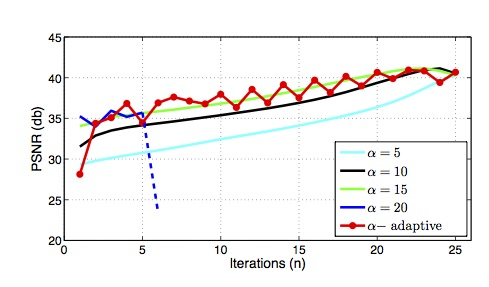
\includegraphics[width = 0.9 \textwidth]{./Diagrams/alpha_accel.jpg}
\caption{Reconstruction performance (expressed in terms of Peak Signal-to-Noise radio) dependence on acceleration coefficients $alpha_n$, for contant value for all iterations $\alpha_n=\alpha$, increasing $\alpha$ brings accelerating convergence, but after some limit, the reconstruction starts to diverge ($\alpha = 20$). Figure taken from \cite{LF-Shearlets} pp. 7}
\label{fig:alpha_accel}
\end{figure}

The approach that we will use and is presented in Algorithm~\ref{alg:lfshearlets1} was proposed by T. Blumensath and M. Davies in 2010 in their article "Normalised Iterative Hard Thresholding; guaranteed stability and performance" \cite{hard-thresholding}. This algorithm applies an iteration-adaptative selection of the parameter given by

$$
\alpha_n=\frac{||\beta_n||_2^2}{||MS^*(\beta_n)||_2^2}
$$

where $\beta_n=S_{\Gamma_n}(y-Mx_n)$ and $S_{\Gamma_n}$ is the shearlet transform decomposition only for coefficients from $\Gamma_n=\textrm{supp}(S(x_n))$. The convergence rate of the adaptative selection is also illustrated in Figure~\ref{fig:alpha_accel} and one can see that the adaptation provides high convergence speed and stable reconstruction we refer to the original paper \cite{hard-thresholding} for a more detailed analysis of the convergence and stability conditions, which for our case are fulfilled using the fact that the $0$-Shearlets system form a Parseval Frame. 

\bigskip

As we discurssed in Subsection~\ref{sec:0-Shearlets} we are not obligated to use all the general shearlet transform atoms, instead we favor the use of atoms which are associated with valid directions in EPI; the support of those atomes is illustrated in Figure~\ref{fig:LFshearlets2f}. The scales of the shearlet transform are constructed in dyadic manner, therefore we are choosing $J = \lceil log_2 d_{max}\rceil$ number of scales. In order to perform this programatically using the software Shearlab.jl in every scale we choose $2^{j+1}+1$ shears ($j=0,\ldots, J-1$) to cover the region.

\bigskip

Finally, in the following subsections we will present the resulting inpainted EPIs of the Church data set, as well as the technique that we use to detect lines in the inpainted EPIs and finally compute the depth map. 

\section{Results of sparse EPIs inpaiting}


\section{Line detection in inpainted EPIs and depth map computation}

